
\section{\genco Model Architecture}


\label{sec:model}

\begin{figure*}
    \centering
    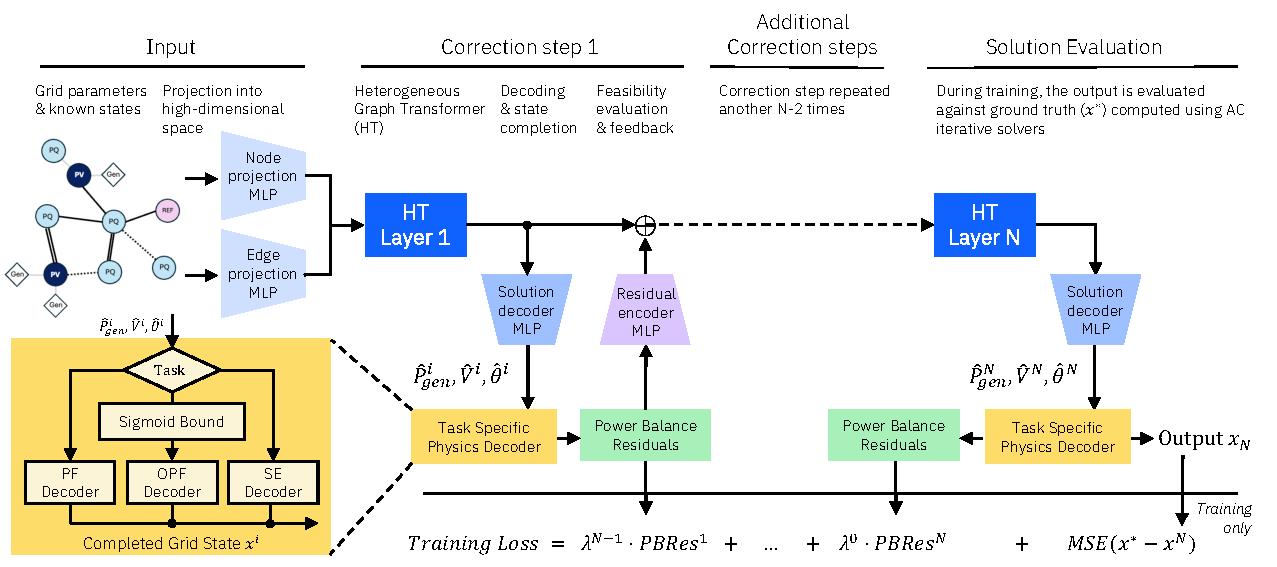
\includegraphics[width=\linewidth]{figures/model/architecture.pdf}
    \caption{Overview of \genco.}
    \label{fig:architecture}
\end{figure*}

In this section, we provide an overview of our model, \genco, which is depicted in \cref{fig:architecture}. The architecture comprises a Multi-Layer Perceptron (MLP)-based input projection layer (\cref{subsec:input}) that projects grid parameters and known states into a high-dimensional latent space, followed by $N$ iterative correction steps (\cref{subsec:correction}). At each step $i$, a heterogeneous Graph Transformer (HT) layer, implemented using the \texttt{HeteroConv}~\cite{Fey_Lenssen_2019, Fey_etal_2025} and \texttt{TransformerConv}~\cite{shi2021maskedlabelpredictionunified} operators, is followed by a Solution Decoder MLP that decodes the primary variables $(\hat{P}_{\text{gen}}^i, \hat{V}^i, \hat{\theta}^i)$. The decoded variables can optionally be bounded by a sigmoid transformation to enforce box constraints before passing through a task-specific physics decoder to obtain a complete intermediate solution containing all injections and voltage states. Power Balance Residuals ($\mathrm{PBRes}^i$) are then computed and fed back through a Residual Encoder MLP, enabling feasibility-aware refinement of the latent representation of the intermediate solution. Finally, the model is trained against ground-truth solutions from classical methods---obtained by Newton--Raphson for PF, interior point methods for OPF, and Weighted Least Squares for SE---by minimizing a loss that combines a supervised distance term to the ground-truth solution with physics-informed residuals accumulated across all correction steps to encourage early feasibility (\cref{subsec:eval}).

\subsection{Input}
\label{subsec:input}

\subsubsection{Grid Parameters and Known States}

The input contains all grid parameters and known operating-state variables as
a heterogeneous directed graph. The graph has two node types—buses and generators—and two edge types: directed branch edges (one per
direction per physical branch) and featureless bus--generator connectivity
edges. We denote by $\mathcal{N}$ the set of buses, $\mathcal{G}$ the set of
generators, and $\mathcal{E}'$ the set of directed branch edges (i.e., one
edge per direction per physical branch). The slack bus is denoted by REF. Bus features encode active and reactive loads, voltage angles and magnitudes, reactive power generation, as well as shunt admittances, voltage limits, and bus-type
indicators (PQ, PV, REF); branch edge features encode admittance parameters, tap ratios,
and thermal and angle limits; generator features encode active and reactive generation,
generation limits, and quadratic dispatch cost coefficients. Variables that
are unknown and must be solved are zeroed out in the input, while known
variables are passed through unchanged. 

\subsubsection{Projection into High-Dimensional Space}

The input projection layer lifts the raw grid features into a shared
high-dimensional latent space. Separate two-layer feed-forward networks
project bus, generator, and branch edge features independently into latent representations
of dimension $H$:
\begin{equation}
    \label{eq:input_proj}
  h_{\text{bus}}^0 \in \mathbb{R}^{|\mathcal{N}| \times H}, \quad
  h_{\text{gen}}^0 \in \mathbb{R}^{|\mathcal{G}| \times H}, \quad
  h_{\text{edge}} \in \mathbb{R}^{|\mathcal{E}'| \times H}.
\end{equation}
Edge embeddings $h_{\text{edge}}$ are computed once and held constant; only bus
and generator embeddings are updated across correction steps.

\subsection{Correction Steps}
\label{subsec:correction}


After projecting the inputs into a higher-dimensional space, \genco operates a series of $N$ correction steps to update the latent representation of a candidate solution for the tasks it solves. This solution is then decoded, evaluated for feasibility of the power balance equations, and updated according to a feedback message.




\subsubsection{Latent Solution Update with an HT Layer}
The GNN layer propagates information between electrically connected components of the grid to produce updated latent representations of the system state at each correction step. An HT layer with $N_h$ attention heads updates bus and generator embeddings by aggregating messages from electrically connected neighbors, using separate attention parameters for each relation type (bus-to-bus, gen-to-bus, bus-to-gen). For bus-to-bus edges, branch embeddings $h_{\text{edge}}$ (computed from the branch admittance and thermal and angle limits) condition the attention mechanism so that electrical coupling strengths modulate information flow. After the GNN update at correction step $i$, each bus and generator has a latent embedding of dimension $N_h \cdot H$:
\begin{equation}
\label{eq:transformer}
z_{\text{bus}}^i \in \mathbb{R}^{|\mathcal{N}| \times (N_h H)}, \qquad
z_{\text{gen}}^i \in \mathbb{R}^{|\mathcal{G}| \times (N_h H)}.
\end{equation}

Thus, for a model with $N$ correction steps, there is one updated bus and generator embedding per node \emph{per step}, encoding both the grid topology and the feasibility feedback injected at the end of the previous correction step (as discussed in \cref{subsec:feedback}).

\subsubsection{Decoding and Solution Completion}
\label{subsubsec:decoding}

At each correction step $i$, a Solution Decoder MLP (with weights shared across all steps) maps the latent embeddings to primary variables
$(\hat{P}_{\mathrm{gen}}^i,\hat{V}^i,\hat{\theta}^i)$.
These variables are optionally projected onto box constraints and then passed through a task-specific physics decoder to construct a complete intermediate solution.

\paragraph{Primary variable decoding.}

A bus-level Solution Decoder MLP maps the bus latent embeddings
$z_{\mathrm{bus}}^i$
to reconstructed voltage magnitudes and angles:
\begin{equation}
\hat{V}^i \in \mathbb{R}^{|\mathcal{N}|},
\qquad
\hat{\theta}^i \in \mathbb{R}^{|\mathcal{N}|}.
\end{equation}

For OPF, a generator-level Solution Decoder MLP maps
$z_{\mathrm{gen}}^i$
to reconstructed active power generations:
\begin{equation}
\hat{P}_{\mathrm{gen}}^i \in \mathbb{R}^{|\mathcal{G}|}.
\end{equation}

For PF and SE, only the voltage state variables are decoded.
All known quantities (e.g., loads and specified generation in PF) are passed through unchanged.

\paragraph{Box constraints.}

For OPF, voltage magnitudes and active generator powers are constrained to their feasible intervals through a sigmoid projection:
\begin{equation}
\hat{x}^i
=
\underline{x}
+
(\overline{x}-\underline{x})
\,\sigma(\tilde{x}^i),
\end{equation}
where $\tilde{x}^i$ denotes the unconstrained decoder output,
$\sigma(\cdot)$ is the sigmoid function,
and $(\underline{x},\overline{x})$ are the lower and upper bounds. No box constraints are imposed for PF or SE.

\paragraph{Physics decoder.}

Given $(\hat{V}^i,\hat{\theta}^i)$, the physics decoder reconstructs
network-implied electrical quantities using the branch admittance model. This applies across all PF, OPF, and SE tasks.
\\\\
Each directed branch edge
$e \in \mathcal{E}'$
is associated with a source bus
$s(e)$
and a target bus
$t(e)$.
The active and reactive power flows leaving the source bus $s(e)$ through edge $e$ are computed as
\begin{align}
\hat{P}_{e}^i
&=
\hat{P}_{e}(\hat{V}^i,\hat{\theta}^i),
\\
\hat{Q}_{e}^i
&=
\hat{Q}_{e}(\hat{V}^i,\hat{\theta}^i).
\end{align}

The corresponding \emph{power-flow-implied injections} are then obtained by summing all outgoing
branch flows:
\begin{align}
\label{eq:inj}
\hat{P}_{\mathrm{inj},k}^i
&=
\sum_{e\,:\,s(e)=k}
\hat{P}_{e}^i,
\\
\hat{Q}_{\mathrm{inj},k}^i
&=
\sum_{e\,:\,s(e)=k}
\hat{Q}_{e}^i.
\end{align}

\paragraph{Recovery of generation variables for OPF.}

Reactive generator powers at PV and REF buses are analytically recovered from the reactive power balance equation:
\begin{equation}
\label{eq:reactive_power_balance}
\hat{Q}_{g,j}^i
=
\hat{Q}_{\mathrm{inj},j}^i
+
Q_{d,j}
-
Q_{\mathrm{shunt},j}(\hat{V}^i),
\end{equation}
where
$Q_{d,j}$ is the reactive demand and
$Q_{\mathrm{shunt},j}(\hat{V}^i)$
denotes the shunt reactive injection computed from the reconstructed voltage.

\paragraph{Recovery of generation variables for PF.}

Reactive generation
$\hat{Q}_{g,j}^i$
is similarly recovered at PV and REF buses using \cref{eq:reactive_power_balance}.
At the REF bus, bus-level active generation
$\hat{P}_{g,\mathrm{REF}}^i$
is recovered from the active power balance equation.
\\\\
A key property of the model is that whenever a variable is analytically recovered from a balance equation,
the corresponding residual component is structurally zero
(\cref{subsec:feedback}). For SE, no generation variables are recovered as the model directly predicts net nodal injections.


\paragraph{Intermediate solution.}

The intermediate solution at correction step $i$ is defined as
\begin{equation}
x^i =
\begin{cases}
[
\hat{V}^i,
\hat{\theta}^i,
\hat{P}_{\mathrm{gen}}^i,
\hat{Q}_{g}^i,
\hat{P}_{\mathrm{flow}}^i,
\hat{Q}_{\mathrm{flow}}^i
]
& \text{(OPF)},
\\[6pt]
[
\hat{V}^i,
\hat{\theta}^i,
\hat{P}_{g,\mathrm{REF}}^i,
\hat{Q}_{g}^i,
\hat{P}_{\mathrm{flow}}^i,
\hat{Q}_{\mathrm{flow}}^i
]
& \text{(PF)},
\\[6pt]
[
\hat{V}^i,
\hat{\theta}^i,
\hat{P}_{\mathrm{inj}}^i,
\hat{Q}_{\mathrm{inj}}^i,
\hat{P}_{\mathrm{flow}}^i,
\hat{Q}_{\mathrm{flow}}^i
]
& \text{(SE)}.
\end{cases}
\end{equation}

For SE, injections are not decomposed into generation and load components.

\subsubsection{Feasibility Evaluation and Feedback}
\label{subsec:feedback}


The feasibility evaluation quantifies the deviation of the intermediate solution $x^i$ from satisfying the nodal power balance equations\footnote{Only active and reactive power-balance residuals are used in the intermediate feedback at each correction step. Other OPF constraints (e.g., thermal limits, branch angle differences, and reactive generation bounds) are not included in this feedback signal. Extending the mechanism to incorporate all constraint types would require combining heterogeneous residuals with additional learned mappings or carefully tuned weightings, substantially increasing hyperparameter complexity, and is left for future work.}, and provides a feedback signal for the next correction step.

\paragraph{Feasibility evaluation using power balance residuals.}
For each bus $k$, we define the per-bus power balance residual vector at correction step $i$ as
\begin{equation}
\mathrm{PBRes}_k^i :=
\begin{bmatrix}
\mathrm{PBRes}_{P,k}^i \\
\mathrm{PBRes}_{Q,k}^i
\end{bmatrix}.
\end{equation}

The active and reactive components are given by:
\begin{align}
\mathrm{PBRes}_{P,k}^i
&:=
\hat{P}_{\mathrm{bus},k}^i
-
\hat{P}_{\mathrm{inj},k}^i
+
P_{\mathrm{shunt},k}(\hat{V}^i),
\nonumber\\
\mathrm{PBRes}_{Q,k}^i
&:=
\hat{Q}_{\mathrm{bus},k}^i
-
\hat{Q}_{\mathrm{inj},k}^i
+
Q_{\mathrm{shunt},k}(\hat{V}^i).
\label{eq:PBRes}
\end{align}
They are computed by comparing (i) the \emph{power-flow-implied injections} $\hat{P}_{\mathrm{inj},k}^i$ and $\hat{Q}_{\mathrm{inj},k}^i$, obtained by summing branch flows (\cref{eq:inj}), and (ii), the \emph{net bus injections}, defined as the difference between bus-level generation and load:
\begin{align}
\label{eq:bus-inj}
\hat{P}_{\mathrm{bus},k}^i &= \hat{P}_{g,k}^i - P_{d,k}, \\
\hat{Q}_{\mathrm{bus},k}^i &= \hat{Q}_{g,k}^i - Q_{d,k}.
\end{align}


For OPF, bus-level generation $\hat{P}_{g,k}$ is obtained by summing the active power generation of all generators connected to bus $k$.\\

Some residual components are structurally zero because the corresponding generation variables are analytically recovered from the power balance equations and therefore satisfy them by construction (e.g., reactive generation at PV buses) (\cref{subsubsec:decoding}). In SE, residuals are evaluated only at buses with available measurements of both generation and load.

\paragraph{Feedback.}
A Residual Encoder MLP maps the residual vector back into the latent space and injects it into the bus embedding before the next GNN layer:

\begin{equation}
h_{\mathrm{bus},k}^{i+1}
=
z_{\mathrm{bus},k}^i
+
\operatorname{MLP}'_{\mathrm{bus}}
\left(
\mathrm{PBRes}_k^i
\right).
\end{equation}

This closes the correction loop: at each step, the model receives an explicit
physics-grounded infeasibility feedback that enables iterative refinement toward
feasible solutions across the $N$ correction steps.

\subsection{Final Solution Evaluation and Training Loss}
\label{subsec:eval}


The training objective combines supervised learning on the final solution with
intermediate self-supervised feasibility regularization through the power balance residuals.

The final prediction is $\hat{x} := x^N$, and the training loss is defined as
\begin{equation}
\label{eq:loss}
\mathcal{L}
=
\mathcal{L}_{\mathrm{supervised}}(x^N, x^*)
+
\sum_{i=1}^{N}
\lambda^{N-i}
\,
\overline{\|\mathrm{PBRes}^i\|}_2,
\end{equation}
where $x^*$ denotes the ground-truth solution obtained from the corresponding classical solver,
$\mathcal{L}_{\mathrm{supervised}}$ is a task-specific supervised loss, and $\overline{\|\mathrm{PBRes}^i\|}_2$ denotes the mean $\ell_2$ norm of the per-bus power balance residual vectors $\mathrm{PBRes}_k^i$ across all buses at correction step $i$. The factor $\lambda^{N-i}$, with $\lambda<1$, is an exponentially increasing weight that places greater emphasis on later correction steps.
The supervised loss is instantiated differently for each task:
MSE on bus- and generator-level variables for OPF,
MSE on bus-level variables for PF,
and MAE on bus- and edge-level variables for SE.\\

\subsection{Training \genco with gridfm-graphkit}


\label{subsec:graphkit}

\genco is implemented and trained using \graphkit\footnote{\url{https://github.com/gridfm/gridfm-graphkit}},
our PyTorch Lightning–based framework for developing neural solvers and grid foundation models. Training and evaluation are configured via YAML files and run through a CLI. The library is optimized for large-scale training. It supports multi-GPU execution, multi-grid training, fine-tuning, and model compilation.\\

\graphkit decouples architecture design from data engineering, training, and evaluation by providing a unified heterogeneous graph structure as a common backbone, shared across PF, OPF, and SE tasks. It handles graph construction, feature normalization, and masking of task-dependent variables, ensuring a consistent representation across models (\cref{fig:motivational_example}). Since new architectures are integrated by defining a forward pass over this standardized graph, it enables straightforward addition and testing of new neural solvers. Further, training components such as losses, optimizers, checkpointing, and logging are implemented in \graphkit. The framework includes power system-specific modules, including physics decoders (\cref{subsubsec:decoding}), power-flow computation, and evaluation of constraint violations and optimality gaps, reducing the need for domain-specific implementation. It also enables direct comparison with classical solvers using precomputed solutions from \datakit.\\

The main benefit brought to the community by \graphkit is benchmarking consistency: data loading, splitting, and evaluation metrics are standardized across models, so that differences arise only from architecture specifications in configuration files while evaluation protocols remain fixed.\\


\begin{boxH}
\paragraph{Takeaways.}
\begin{itemize}
\item \genco is a unified iterative correction architecture that maps grid states to PF/OPF/SE solutions via $N$ correction steps in a high-dimensional latent space, learned from precomputed solutions.
\item Each iteration decodes full physical states and is refined using power-balance residuals, providing physics-grounded infeasibility feedback (self-supervision).
\item The architecture combines learned message passing with sparse attention with a task-specific physics decoder that performs solution completion via power-flow equations and enforces OPF box constraints through sigmoid projections.
\end{itemize}
\end{boxH}